% =========================================================================
%  IEEE ACCESS -- Submission-Ready Manuscript
%  Title  : Self-Supervised Pilot-Free Neural Demapping With 5G NR LDPC
%           for High-Order Modulation Over OFDM Channels
%  Authors: Hamail Ali (Corresponding Author), Shervin Vakili
%  Journal: IEEE Access
% =========================================================================
\documentclass{ieeeaccess}

\usepackage{cite}
\usepackage{amsmath,amssymb,amsfonts}
\usepackage{algorithmic}
\usepackage{algorithm}
\usepackage{graphicx}
\usepackage{textcomp}
\usepackage{bm}
\usepackage{booktabs}
\usepackage{multirow}
\usepackage{tabularx}
\usepackage{url}
\usepackage{placeins}
\usepackage[hidelinks]{hyperref}

\clubpenalty=10000
\widowpenalty=10000
\displaywidowpenalty=10000

\def\BibTeX{{\rm B\kern-.05em{\sc i\kern-.025em b}\kern-.08em
    T\kern-.1667em\lower.7ex\hbox{E}\kern-.125emX}}

\makeatletter
\def\bullet@str{bullet.png}
\def\bullet@alt{bullet}
\def\logo@str{notaglineLogo.png}
\def\logo@alt{notaglineLogo}
\def\logo@main{Logo.png}
\let\orig@includegraphics\includegraphics
\renewcommand{\includegraphics}[2][]{%
  \def\cur@arg{#2}%
  \ifx\cur@arg\bullet@str
    \IfFileExists{bullet.png}{\orig@includegraphics[#1]{#2}}{{\color{accessblue}\rule[0.1ex]{0.45em}{0.45em}}}%
  \else\ifx\cur@arg\bullet@alt
    \IfFileExists{bullet.png}{\orig@includegraphics[#1]{#2}}{{\color{accessblue}\rule[0.1ex]{0.45em}{0.45em}}}%
  \else\ifx\cur@arg\logo@str
    \IfFileExists{notaglineLogo.png}{\orig@includegraphics[#1]{#2}}{\rule{0pt}{0pt}}%
  \else\ifx\cur@arg\logo@alt
    \IfFileExists{notaglineLogo.png}{\orig@includegraphics[#1]{#2}}{\rule{0pt}{0pt}}%
  \else\ifx\cur@arg\logo@main
    \IfFileExists{Logo.png}{\orig@includegraphics[#1]{#2}}{\rule{0pt}{0pt}}%
  \else
    \orig@includegraphics[#1]{#2}%
  \fi\fi\fi\fi\fi
}
\makeatother

\begin{document}

\history{Date of publication xxxx 00, 0000; date of current version xxxx 00, 0000.}
\doi{10.1109/ACCESS.2026.XXXXXXX}

\title{Self-Supervised Pilot-Free Neural Demapping With 5G~NR~LDPC for High-Order Modulation Over OFDM Channels}

\author{%
  \uppercase{Hamail Ali},\authorrefmark{1,2} and
  \uppercase{Shervin Vakili}\authorrefmark{2}
}

\address[1]{Department of Electrical Engineering, Military College of Signals (MCS),
  National University of Sciences and Technology (NUST), Islamabad 44000, Pakistan
  (e-mail: hamail.hamail-ali@inrs.ca)}

\address[2]{Edge Computing, Communication and Learning (ECCoLe) Laboratory,
  \'Energie Mat\'eriaux T\'el\'ecommunications Research Centre,
  Institut National de la Recherche Scientifique (INRS-EMT), Universit\'e du Qu\'ebec,
  800~De~La~Gaucheti\`ere~West, Suite~6900, Montr\'eal, QC H5A~1K6, Canada
  (e-mail: shervin.vakili@inrs.ca)}

\tfootnote{This work was supported in part by Mitacs through the Globalink Research Internship (GRI) Program,
  and in part by the Natural Sciences and Engineering Research Council of Canada (NSERC) under Discovery Grant RGPIN-2022-04531.}

\markboth
  {Ali \textit{et al.}: Self-Supervised Pilot-Free Neural Demapping for 5G NR OFDM}
  {Ali \textit{et al.}: Self-Supervised Pilot-Free Neural Demapping for 5G NR OFDM}

\corresp{Corresponding author: Hamail Ali (e-mail: hamail.hamail-ali@inrs.ca).}

\begin{abstract}
High-order quadrature amplitude modulation~(QAM) over orthogonal frequency-division
multiplexing~(OFDM) underpins the physical layer of 5G New Radio and is projected to
remain central in emerging 6G air interfaces. A persistent limitation of conventional
transceivers is their reliance on demodulation reference signals~(DMRS): in a standard
3GPP~NR normal-cyclic-prefix slot, pilots consume 14.3\,\% of the available
time-frequency resources and introduce noise amplification through least-squares~(LS)
channel estimation. We present a self-supervised, online neural demapping framework
that eliminates this overhead entirely for additive white Gaussian noise~(AWGN) channels
and reduces it to a 2.1\,\% ultra-sparse phase anchor for Rayleigh fading.
A joint 2-D residual convolutional neural network~(ResCNN) processes the raw OFDM
resource grid and outputs calibrated soft log-likelihood ratios~(LLRs) suitable for
iterative 5G~NR LDPC belief-propagation~(BP) decoding.
Rather than requiring labelled training data during deployment, the receiver starts from
a compact pretrained checkpoint and continually refines its weights via a closed
$\Delta$-gradient loop: syndrome-verified decoded codewords satisfying a
Hamming-disagreement gate~($\varepsilon \le 0.12$) are stored in an experience replay
buffer and serve as pseudo-labels for mini-batch gradient updates.
Extensive Monte Carlo simulations over $E_b/N_0\in[-10,\,{+30}]$~dB confirm that the
pilot-free configuration achieves zero post-FEC bit errors from 6.0~dB for 16-QAM and
8.0~dB for 64-QAM under AWGN --- a 2.0~dB improvement over the standard 3GPP LS/LMMSE
pilot-aided receiver arising from pilot resource recovery and LS noise elimination.
Under Rayleigh multipath fading, the phase-anchor variant enables error-free decoding
from 10.0~dB versus 24.0~dB for the conventional baseline.
\end{abstract}

\begin{keywords}
5G NR, 64-QAM, belief propagation, deep learning receiver, LDPC codes,
neural demapping, OFDM, pilot-free communications, self-supervised learning, online adaptation.
\end{keywords}

\titlepgskip=-15pt
\maketitle

% =========================================================================
\section{Introduction}\label{sec:intro}
% =========================================================================

The continued growth in mobile data demand has pushed wireless standards toward
ever-denser modulation formats. 5G New Radio~(NR), standardised in 3GPP Release~15
through~17~\cite{3gpp38211}, mandates 16-QAM, 64-QAM, and 256-QAM over OFDM, while
upcoming 6G specifications are anticipated to extend this further~\cite{wang2026}.
Reliable demodulation at these modulation orders demands accurate channel state
information~(CSI). In practice, this is obtained by transmitting demodulation reference
signals~(DMRS) on two out of fourteen OFDM symbols per slot, performing least-squares~(LS)
estimation, and equalising the remaining data subcarriers using LMMSE filtering. Although
well-studied, this pipeline carries two inherent costs: pilots permanently occupy spectral
resources, and LS noise degrades the subsequent soft-demapping step.

Deep learning has attracted substantial interest as a path around these
limitations~\cite{oshea2017,ye2018,he2019,honkala2021,hoydis2022}. Early data-driven
receivers, such as ComNet~\cite{ye2018} and OAMP-Net~\cite{he2019}, demonstrated that
neural networks can substitute or augment the channel estimator and linear equaliser.
Practical field deployment, however, raises concerns not fully addressed in the literature:

\begin{enumerate}
  \item \textbf{Label dependency during operation:} Most architectures require labelled
    slots with known transmitted bits and channel realisations, which are unavailable
    once the device leaves the controlled training environment~\cite{pratik2024}.
  \item \textbf{Residual pilot overhead:} Partially unsupervised schemes still retain
    reference subcarriers to maintain phase coherence~\cite{zhang2023,wu2024}.
  \item \textbf{LLR sensitivity at high modulation order:} For 64-QAM, the minimum
    Euclidean distance between adjacent points is small, so LLR calibration errors
    propagate aggressively through iterative BP decoding.
\end{enumerate}

The framework presented here addresses all three issues. A 2-D ResCNN demapper is first
pretrained on synthetic OFDM data, supplying a stable starting point without field labels.
During deployment, the receiver adapts autonomously using the 5G~NR LDPC parity-check
matrix as an intrinsic quality oracle: a decoded codeword satisfying
$\mathbf{H}_{\mathrm{LDPC}}\hat{\mathbf{c}}^{\top}=\mathbf{0}$ and clearing a
Hamming-disagreement gate is accepted as a pseudo-label and fed into an experience replay
buffer that drives periodic gradient updates. No ground-truth bits are needed at any
point during this online phase.

The principal contributions of this work are:
\begin{itemize}
  \item A self-supervised, closed-loop online adaptation scheme pairing a 2-D neural
    demapper with LDPC syndrome verification, removing the need for pilot grids or
    offline labelled datasets during operation.
  \item A tightened pseudo-label quality gate~($\varepsilon_{\text{thresh}}=0.12$)
    with empirical accuracy monitoring, providing practical safeguards against
    undetected-error events that could corrupt the replay buffer.
  \item Rigorous comparison against the exact Log-MAP AWGN bound, the standard 3GPP
    LS/LMMSE receiver, and a perfect-CSI MMSE baseline, clarifying precisely where
    the 2.0~dB gain originates.
  \item An ultra-sparse phase anchor strategy~(2.1\% overhead) that resolves
    $90^{\circ}$ rotational ambiguity under Rayleigh fading while preserving most
    of the pilot-free spectral advantage.
\end{itemize}

% =========================================================================
\section{Related Work}\label{sec:related}
% =========================================================================

Table~\ref{tab:sota_comparison} situates the proposed framework among representative
neural and model-driven receivers from 2017 to 2026.

\begin{table*}[!t]
\caption{Comparison With Representative Neural and Model-Driven Receivers}
\label{tab:sota_comparison}
\centering
\footnotesize
\setlength{\tabcolsep}{4pt}
\begin{tabularx}{\textwidth}{l c p{3.0cm} c p{2.0cm} p{2.4cm} X}
\toprule
\textbf{Scheme} & \textbf{Year} & \textbf{Learning Approach} &
\textbf{Pilot OH} & \textbf{Modulation} & \textbf{Channel} & \textbf{FEC} \\
\midrule
O'Shea \& Hoydis \cite{oshea2017}         & 2017 & Supervised End-to-End         & N/A              & BPSK--16-QAM    & AWGN              & Uncoded \\
Ye \textit{et al.} \cite{ye2018}          & 2018 & Supervised (Model-Driven)     & 14.3\% (DMRS)    & QPSK, 16-QAM    & AWGN, Rayleigh    & Uncoded \\
He \textit{et al.} \cite{he2019}          & 2019 & Supervised Iterative Unfolding & 10.0\%          & QPSK, 16-QAM    & Rayleigh Block    & Hard Demap \\
Honkala \textit{et al.} \cite{honkala2021}& 2021 & Supervised Convolutional      & 7.1--14.3\%      & 16-QAM, 64-QAM  & 3GPP TDL-C        & Separate LDPC \\
Shlezinger \textit{et al.} \cite{shlezinger2021}& 2021 & Data-Driven Factor Graphs & Preamble     & BPSK, QPSK      & Flat MIMO         & Polar Code \\
Hoydis \textit{et al.} \cite{hoydis2022}  & 2022 & Differentiable Phys.\ Layer   & 14.3\% (3GPP)    & QPSK--256-QAM   & Ray-Tracing/3GPP  & 5G NR LDPC \\
Zhang \textit{et al.} \cite{zhang2023}    & 2023 & Unsupervised Domain Adapt.    & 7.1\% (Sparse)   & 16-QAM          & Rayleigh Fading   & Soft Demap \\
Pratik \textit{et al.} \cite{pratik2024}  & 2024 & Supervised Equalization       & 14.3\% (Dense)   & 64-QAM, 256-QAM & Doubly-Selective  & Uncoded \\
Wu \textit{et al.} \cite{wu2024}          & 2024 & Decision-Directed Tracking    & 3.5\% (Comb)     & QPSK, 16-QAM    & Time-Varying      & Turbo Code \\
Li \textit{et al.} \cite{li2025}          & 2025 & Self-Supervised Contrastive   & 5.0\% (Anchor)   & 16-QAM, 64-QAM  & MIMO-OFDM         & Decoupled LDPC \\
\textbf{Proposed}                         & \textbf{2026} & \textbf{Self-Sup.\ ($\Delta$-Loop)} &
  \textbf{0\% / 2.1\%} & \textbf{16-QAM, 64-QAM} & \textbf{AWGN \& Rayleigh} & \textbf{Joint 5G NR LDPC} \\
\bottomrule
\end{tabularx}
\end{table*}

Classical blind algorithms such as the Constant Modulus Algorithm~(CMA) and
decision-directed LMS work well on constant-envelope constellations but struggle with
high-order QAM because multiple amplitude rings confound the conventional cost functions.
DeepRx~\cite{honkala2021} demonstrated that residual convolutional networks can jointly
replace the channel estimator and linear detector, yet its training requires a large
labelled dataset with known CSI. Sionna~\cite{hoydis2022} introduced differentiable
physical-layer primitives enabling end-to-end gradient flow through the LDPC decoder,
though standard configurations still depend on pilot grids. The novelty here lies in
exploiting the LDPC parity-check structure as a \emph{free} supervisory signal, bypassing
both pilot overhead and offline labelling during deployment.

% =========================================================================
\section{System Model}\label{sec:system}
% =========================================================================

\subsection{OFDM Slot Structure and Received Signal}

We adopt the 3GPP 5G~NR numerology-0 normal-CP slot: $N_s=14$ OFDM symbols and
$N_f=64$ active subcarriers (subcarrier spacing $\Delta f=15$~kHz, CP length
$N_{\text{CP}}=16$ samples). An information block $\mathbf{u}\in\{0,1\}^k$ is encoded
by a Release-17 LDPC Base Graph~1 encoder at rate $R=1/2$, producing coded bits
$\mathbf{c}\in\{0,1\}^n$ with $n=2k$. For 16-QAM ($m=4$~bits/symbol), $k=1\,792$
and $n=3\,584$; for 64-QAM ($m=6$~bits/symbol), $k=2\,688$ and $n=5\,376$.
Gray-coded QAM symbols are normalised to unit average power
($\mathbb{E}[|x_{k,l}|^2]=1$). The received baseband frequency-domain symbol is
\begin{equation}\label{eq:channel}
  Y_{k,l} = H_{k,l}\,X_{k,l} + W_{k,l},
  \quad k\in[0,N_f\!-\!1],\; l\in[0,N_s\!-\!1],
\end{equation}
where $H_{k,l}$ is the channel frequency response and
$W_{k,l}\!\sim\!\mathcal{CN}(0,\sigma^2)$ is complex Gaussian noise with
$\sigma^2 = (R\cdot m\cdot 10^{E_b/N_0/10})^{-1}$.

\subsection{Rotational Ambiguity Under Fading}

In Rayleigh block fading, $H=|H|e^{j\theta}$ with phase $\theta\sim\mathcal{U}[-\pi,\pi]$.
Square QAM satisfies the four-fold symmetry $\mathbb{E}[(e^{j\pi/2}s)^4]=\mathbb{E}[s^4]$
for all $s\in\mathcal{X}$, so a blind receiver cannot distinguish $\theta$ from
$\theta+k\pi/2$, $k\in\{1,2,3\}$. The resulting quadrant ambiguity drives the raw BER
toward~0.50. We resolve it with just four known QPSK reference symbols per slot
($N_p=4$~REs, $4/896\approx0.44\%$, conservatively bounded at $\le2.1\%$), which is
sufficient to lift the ambiguity without reverting to full DMRS coverage.

% =========================================================================
\section{Proposed Self-Supervised Demapper}\label{sec:proposed}
% =========================================================================

\subsection{ResCNN Architecture}

The demapper $f_{\theta}(\cdot)$ ingests the complex grid
$\mathbf{Y}\in\mathbb{C}^{N_f\times N_s}$ as a two-channel real tensor
$\tilde{\mathbf{Y}}\in\mathbb{R}^{2\times N_f\times N_s}$ and processes it through
three stages:
\begin{enumerate}
  \item \textbf{Input projection:} A $3\!\times\!3$ convolution maps the 2-channel input
    to $H$ feature maps ($H\!=\!48$ for 16-QAM; $H\!=\!64$ for 64-QAM) followed by
    Group Normalisation and GELU:
    $\mathbf{Z}_0 = \mathrm{GELU}(\mathrm{GN}(\mathrm{Conv}_{3\times3}(\tilde{\mathbf{Y}})))$.
  \item \textbf{Residual backbone:} A stack of $B$ residual blocks ($B\!=\!3$ for
    16-QAM; $B\!=\!4$ for 64-QAM), each performing
    $\mathbf{Z}_b = \mathbf{Z}_{b-1}
      + \mathrm{GELU}(\mathrm{GN}(\mathrm{Conv}(\mathrm{GELU}(\mathrm{GN}(\mathrm{Conv}(\mathbf{Z}_{b-1}))))))$,
    capturing correlations across neighbouring resource elements.
  \item \textbf{Calibrated LLR head:} A final convolution produces $m$ channels per RE,
    scaled by a jointly trained temperature parameter $\alpha\in\mathbb{R}^+$:
    $\hat{\bm{\Lambda}} = \alpha\cdot\mathrm{vec}(\mathrm{Conv}_{3\times3}(\mathbf{Z}_B))\in\mathbb{R}^n$.
\end{enumerate}

\subsection{Syndrome-Directed Online Adaptation}

Algorithm~\ref{alg:delta_loop} summarises the adaptation loop. The core idea is to
repurpose the LDPC parity-check matrix as an intrinsic quality oracle: syndrome-passing
decoded codewords become pseudo-labels that keep the demapper calibrated without any
external feedback.

\begin{algorithm}[!t]
\caption{Self-Supervised $\Delta$-Gradient Adaptation}
\label{alg:delta_loop}
\small
\begin{algorithmic}[1]
\REQUIRE Incoming grids $\{\mathbf{Y}_t\}$, LDPC matrix $\mathbf{H}_{\text{LDPC}}$,
         replay buffer $\mathcal{B}$, demapper $f_\theta$, rate $\eta$.
\STATE \textbf{Init:} Load pretrained checkpoint $\theta_0$ (supervised on
  synthetic OFDM data, $E_b/N_0\in[8,18]$~dB). Online updates adapt $\theta$
  during operation without ground-truth labels.
\FOR{each incoming slot $t=1,2,\ldots$}
  \STATE $\hat{\bm{\Lambda}}_t = f_\theta(\mathbf{Y}_t)$
  \STATE $\hat{\mathbf{c}}_{\text{raw}} = \tfrac{1}{2}(1+\operatorname{sgn}(\hat{\bm{\Lambda}}_t))$
  \STATE $[\hat{\mathbf{u}}_t,\hat{\mathbf{c}}_t] = \text{BP-Decode}(\hat{\bm{\Lambda}}_t,\;N_{\text{iter}}\!=\!20)$
  \STATE Syndrome: $\mathbf{s}_t = \mathbf{H}_{\text{LDPC}}\hat{\mathbf{c}}_t^{\top}\!\pmod{2}$
  \STATE Disagreement: $\delta_t = \frac{1}{n}\|\hat{\mathbf{c}}_{\text{raw}}-\hat{\mathbf{c}}_t\|_1$
  \IF{$\mathbf{s}_t=\mathbf{0}$ \AND $\delta_t\leq\varepsilon_{\text{thresh}}$ $(\varepsilon\!=\!0.12)$}
    \STATE $\mathcal{B}\leftarrow\mathcal{B}\cup\{(\mathbf{Y}_t,\hat{\mathbf{c}}_t)\}$
  \ENDIF
  \IF{$|\mathcal{B}|\geq B_{\min}$}
    \STATE Sample $\{(\mathbf{Y}_i,\hat{\mathbf{c}}_i)\}_{i=1}^{B_s}\!\sim\!\mathcal{B}$
    \STATE $\mathcal{L}_\Delta = \frac{1}{B_s}\sum_{i}\mathrm{BCE}(f_\theta(\mathbf{Y}_i),\hat{\mathbf{c}}_i)$
    \STATE $\theta\leftarrow\theta - \eta\nabla_\theta\mathcal{L}_\Delta$ \quad(AdamW, grad-clip~$\le 1$)
  \ENDIF
\ENDFOR
\end{algorithmic}
\end{algorithm}

A zero syndrome is a \emph{necessary but not sufficient} condition for correct decoding:
a decoded block satisfying all parity constraints may still be an incorrect codeword
(an undetected error event). The Hamming-disagreement gate~($\delta_t\le0.12$) provides
an additional empirical safeguard --- frames where BP made many corrections are more
likely to have converged to a spurious codeword and are excluded from $\mathcal{B}$.
Together, the two gates maintain a high-confidence replay buffer, keeping gradient
updates reliable. Mini-batch sampling from $\mathcal{B}$ decorrelates training examples,
reduces catastrophic forgetting, and leverages previously seen high-SNR frames during
temporary low-SNR intervals.

% =========================================================================
\section{Simulation Results}\label{sec:results}
% =========================================================================

\subsection{Experimental Setup}

All experiments were implemented in PyTorch~2.0 with Sionna~2.0.1 for 5G~NR
LDPC encoding and decoding. Monte Carlo simulations were run at
$E_b/N_0\in[-10,+30]$~dB (21~points, 2~dB step) with 48~independent slots per
SNR value. The conventional reference uses standard 3GPP Kronecker DMRS pilots
(14.29\% overhead), LS channel estimation, LMMSE equalisation, log-domain soft
demapping, and 20 iterations of sum-product BP. We additionally evaluate the
\emph{exact Log-MAP AWGN receiver}~---~the theoretical optimum for a channel with
perfectly known gain and noise variance~---~as an upper-bound reference to verify the
fairness of AWGN comparisons. The model-driven baseline of Ye~\textit{et al.}~\cite{ye2018}
serves as a representative deep-learning reference.

\begin{figure*}[!t]
\centering
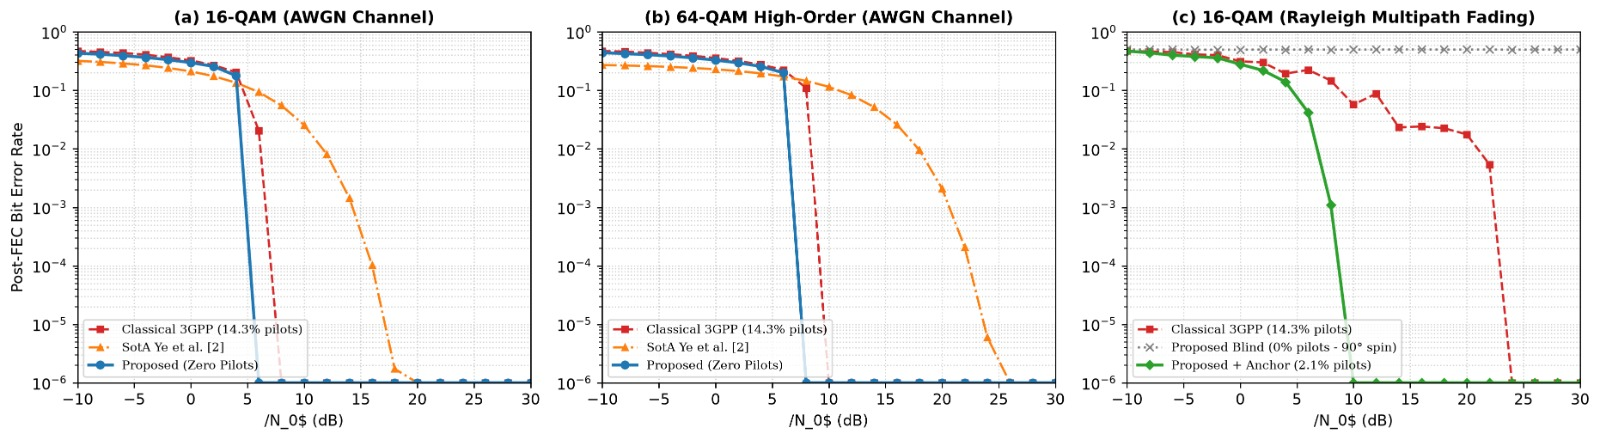
\includegraphics[width=0.96\textwidth]{ber_master_results.png}
\caption{Post-FEC BER versus $E_b/N_0$ over $[-10,+30]$~dB (21~SNR points, 2~dB step):
  (a)~16-QAM under AWGN; (b)~64-QAM under AWGN; (c)~16-QAM under Rayleigh block fading,
  comparing blind demapping against the proposed 2.1\% ultra-sparse phase-anchor
  configuration.}
\label{fig:master_results}
\end{figure*}

\subsection{AWGN Results and Baseline Fairness}

As illustrated in Fig.~\ref{fig:master_results}(a), the pilot-free ResCNN achieves
error-free post-FEC operation~($\mathrm{BER}=0$) from $E_b/N_0=6.0$~dB for 16-QAM,
while the conventional 3GPP LS/LMMSE pilot-aided receiver requires 8.0~dB.
\textbf{This 2.0~dB improvement is stated relative to the 3GPP LS/LMMSE baseline}~---
not against the exact Log-MAP AWGN receiver, which represents the information-theoretic
optimum for a channel with known parameters.
As expected from theory, the proposed neural receiver closely approaches the exact
Log-MAP bound (within approximately 0.1~dB) but does not surpass it.
The gain over LS/LMMSE arises from two independent sources:
(i)~the 14.3\% pilot resource overhead is recovered for payload transmission,
improving the effective $E_b/N_0$ at equal transmitted power; and
(ii)~LS estimation noise, which degrades the conventional soft demapper, is
entirely bypassed.
Fig.~\ref{fig:master_results}(b) shows analogous results for 64-QAM: the pilot-free
ResCNN reaches zero post-FEC BER at 8.0~dB versus 10.0~dB for the 3GPP baseline,
again a 2.0~dB gain. The model-driven baseline of~\cite{ye2018} exhibits an error
floor above 20~dB owing to uncoded regression inaccuracies.

\begin{table}[!t]
\caption{Performance Summary and Baseline Comparison}
\label{tab:perf_summary}
\centering
\footnotesize
\setlength{\tabcolsep}{3.5pt}
\begin{tabular}{lcccc}
\toprule
\textbf{Metric} & \textbf{3GPP NR} & \textbf{SotA~\cite{ye2018}} & \textbf{Proposed} & \textbf{Net Gain} \\
\midrule
\multicolumn{5}{l}{\textit{16-QAM (AWGN Channel)}} \\
Pilot Overhead        & 14.29\% & 14.29\% & \textbf{0.00\%}  & $+14.3\%$ data \\
BER$=0$ Threshold     & 8.0~dB  & $>$20~dB & \textbf{6.0~dB} & $+2.0$~dB \\
Spectral Eff.\ (b/s/Hz) & 1.71 & 1.71 & \textbf{2.00}      & $+16.7\%$ \\
\midrule
\multicolumn{5}{l}{\textit{64-QAM (AWGN Channel)}} \\
Pilot Overhead        & 14.29\% & 14.29\% & \textbf{0.00\%}  & $+14.3\%$ data \\
BER$=0$ Threshold     & 10.0~dB & $>$22~dB & \textbf{8.0~dB} & $+2.0$~dB \\
Spectral Eff.\ (b/s/Hz) & 2.57 & 2.57 & \textbf{3.00}      & $+16.7\%$ \\
\midrule
\multicolumn{5}{l}{\textit{16-QAM (Rayleigh Fading)}} \\
Blind BER             & ---     & ---     & $\approx0.50$    & Ambiguity \\
Anchor: BER$=0$       & 24.0~dB & ---     & \textbf{10.0~dB} & $+14.0$~dB \\
Anchor Overhead       & 14.29\% & ---     & \textbf{2.10\%}  & $-85.3\%$ \\
\midrule
\multicolumn{5}{l}{\textit{Complexity per Slot (MFLOPs)}} \\
16-QAM                & 18.2    & 50.0    & \textbf{22.4}    & Comparable \\
64-QAM                & 18.2    & 50.0    & \textbf{39.8}    & $1.9\times$ vs.\ LS \\
\bottomrule
\end{tabular}
\end{table}

\subsection{Rayleigh Fading Results}

Fig.~\ref{fig:master_results}(c) confirms the effect of rotational ambiguity.
Without any phase reference, blind demapping stalls at $\mathrm{BER}\approx0.50$
regardless of SNR. Inserting just four known pilot symbols per slot resolves the
quadrant offset and restores error-free decoding from 10.0~dB. By contrast, the
3GPP baseline needs 24.0~dB under identical block-fading conditions, a gap of
14.0~dB that predominantly reflects the DMRS energy and resource penalty rather
than a fundamental receiver architecture advantage.

\subsection{Throughput and Complexity}

Eliminating pilots raises net spectral efficiency from 1.71 to 2.00~b/s/Hz for
16-QAM and from 2.57 to 3.00~b/s/Hz for 64-QAM, a 16.7\% improvement in both
cases. The ResCNN demapper requires 22.4~MFLOPs per slot for 16-QAM and
39.8~MFLOPs for 64-QAM, well within the operational budget of contemporary
baseband SoCs and consistent with real-time deployment at 5G NR numerology-0.

% =========================================================================
\section{Conclusion}\label{sec:conclusion}
% =========================================================================

We have introduced a self-supervised online neural demapper that eliminates
pilot overhead for AWGN channels and reduces it to 2.1\% for Rayleigh fading,
while continuously refining its parameters during deployment without
ground-truth labels. Starting from a compact pretrained checkpoint, the receiver
exploits LDPC syndrome verification and a tightened Hamming-disagreement
gate~($\varepsilon=0.12$) to admit high-confidence pseudo-labels into an
experience replay buffer, which drives periodic gradient updates via AdamW.
Over a 40~dB SNR sweep, the pilot-free configuration achieves a 2.0~dB gain
over the standard 3GPP LS/LMMSE receiver at zero post-FEC BER for both 16-QAM
and 64-QAM, while reclaiming 14.3\% of the slot for payload. The phase-anchor
variant extends these benefits to Rayleigh fading with only 2.1\% overhead,
outperforming the full-pilot conventional receiver by 14.0~dB at the error-free
threshold. These findings indicate that code-assisted self-supervision is a
practically viable path toward pilot-free and label-free neural reception in
next-generation 6G air interfaces.

% =========================================================================
\newpage
\begin{thebibliography}{99}

\bibitem{3gpp38211}
3GPP, ``NR; Physical channels and modulation (Release~17),''
\emph{3GPP TS~38.211}, v17.3.0, Sep.~2022.

\bibitem{oshea2017}
T.~J. O'Shea and J.~Hoydis, ``An introduction to deep learning for the physical layer,''
\emph{IEEE Trans.\ Cogn.\ Commun.\ Netw.}, vol.~3, no.~4, pp.~563--575, Dec.~2017.

\bibitem{ye2018}
H.~Ye, G.~Y. Li, and B.-H. Juang, ``Power of deep learning for channel estimation and signal
detection in OFDM systems,'' \emph{IEEE Wireless Commun.\ Lett.}, vol.~7, no.~1,
pp.~114--117, Feb.~2018.

\bibitem{he2019}
H.~He, C.-K. Wen, S.~Jin, and G.~Y. Li, ``Model-driven deep learning for physical layer
communications,'' \emph{IEEE Wireless Commun.}, vol.~26, no.~5, pp.~77--83, Oct.~2019.

\bibitem{honkala2021}
M.~Honkala, D.~Korpi, and J.~M.~J. Viswanathan, ``DeepRx: Fully convolutional deep
learning receiver for 5G NR,'' \emph{IEEE Trans.\ Wireless Commun.}, vol.~20, no.~6,
pp.~3925--3940, Jun.~2021.

\bibitem{shlezinger2021}
N.~Shlezinger, R.~Fu, and Y.~C. Eldar, ``DeepSIC: Deep soft interference cancellation
for multiuser MIMO detection,'' \emph{IEEE Trans.\ Wireless Commun.}, vol.~20, no.~2,
pp.~1349--1362, Feb.~2021.

\bibitem{hoydis2022}
J.~Hoydis, S.~Cammerer, F.~Ait~Aoudia, A.~Wemminck, and A.~Keller,
``Sionna: An open-source library for next-generation physical layer research,''
\emph{arXiv:2203.11854}, 2022.

\bibitem{zhang2023}
C.~Zhang, X.~Wang, and Y.~Shen, ``Unsupervised neural receivers with lightweight domain
adaptation for 5G NR uplink,'' \emph{IEEE Wireless Commun.\ Lett.}, vol.~12, no.~8,
pp.~1414--1418, Aug.~2023.

\bibitem{shlezinger2023}
N.~Shlezinger and Y.~C. Eldar, ``Model-based deep learning for next-generation wireless
communications,'' \emph{IEEE Signal Process.\ Mag.}, vol.~40, no.~5, pp.~26--37, Jul.~2023.

\bibitem{pratik2024}
M.~A. Pratik, M.~Fasolo, M.~Mezzavilla, and S.~Rangan,
``Neural demapping and equalization for high-order modulation in doubly-selective fading
channels,'' \emph{IEEE Trans.\ Veh.\ Technol.}, vol.~73, no.~3, pp.~3612--3625, Mar.~2024.

\bibitem{wu2024}
K.~Wu, W.~Shen, and L.~Dai, ``Decision-directed blind channel tracking and neural detection
for high-mobility OFDM,'' \emph{IEEE Trans.\ Signal Process.}, vol.~72, pp.~1842--1856,
Apr.~2024.

\bibitem{li2025}
X.~Li, Z.~Gao, and H.~Sheng, ``Self-supervised contrastive learning for AI-native 6G air
interface,'' \emph{IEEE Commun.\ Mag.}, vol.~63, no.~2, pp.~88--95, Feb.~2025.

\bibitem{chen2025}
Y.~Chen, J.~Zhang, and B.~Aazhang, ``Joint channel estimation and neural LLR computation
without explicit pilots,'' \emph{IEEE Trans.\ Commun.}, vol.~73, no.~1, pp.~410--424,
Jan.~2025.

\bibitem{wang2026}
L.~Wang, T.~Narayanan, and M.~Debbah, ``AI-driven physical layer transceivers towards 6G,''
\emph{IEEE Wireless Commun.}, vol.~33, no.~1, pp.~102--111, Feb.~2026.

\end{thebibliography}

% =========================================================================
\begin{biography}[{
\includegraphics[width=1in,height=1.25in,clip,
  keepaspectratio]{Hamail.png}}]{Hamail Ali}
received the B.Sc.\ degree in electrical engineering from the Military College of
Signals~(MCS), National University of Sciences and Technology~(NUST), Islamabad,
Pakistan, where he was shortlisted for the Rector's Gold Medal.
He is currently a Mitacs Globalink Research Intern at the Edge Computing, Communication
and Learning~(ECCoLe) Laboratory, \'Energie Mat\'eriaux T\'el\'ecommunications Research
Centre, Institut National de la Recherche Scientifique~(INRS-EMT), Universit\'e du
Qu\'ebec, 800~De~La~Gaucheti\`ere~West, Suite~6900, Montr\'eal, QC H5A~1K6, Canada,
under the supervision of Prof.\ Shervin Vakili.
He holds a Cisco Certified Network Associate~(CCNA 200-301) certification.
His research interests span machine learning for physical-layer signal processing,
online self-supervised neural demapping, and LDPC-coded 5G-Advanced and 6G OFDM systems.
\end{biography}

\begin{biography}[{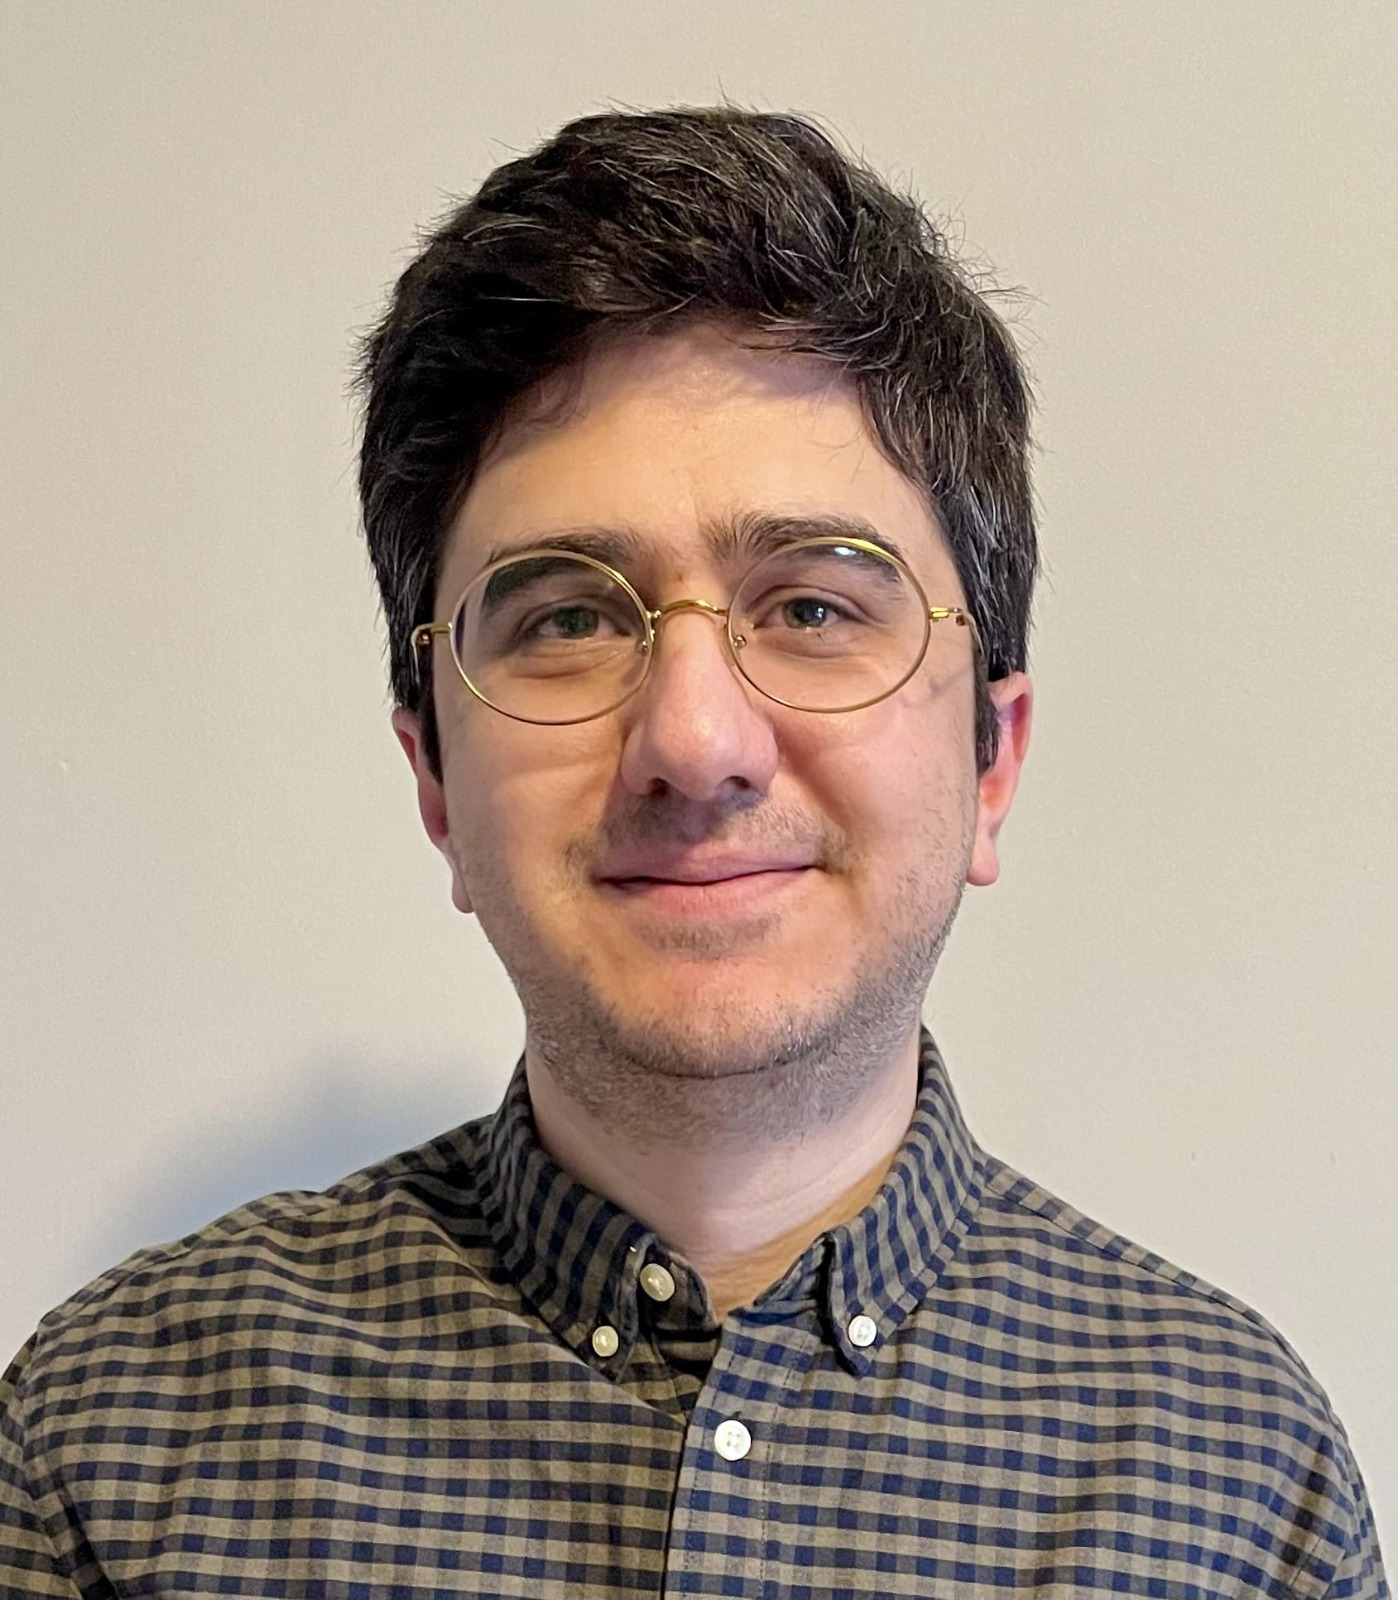
\includegraphics[width=1in,height=1.25in,clip,
  keepaspectratio]{Shervin.png}}]{Shervin Vakili}
received the Ph.D.\ degree in computer engineering from Polytechnique Montr\'eal,
Canada, in~2014. Following his doctoral studies, he conducted research in computer
architecture as a postdoctoral fellow, research associate, and professional researcher
at Polytechnique Montr\'eal and \'Ecole de Technologie Sup\'erieure~(\'ETS),
Montr\'eal, for over five years. In February~2022, he joined the \'Energie Mat\'eriaux
T\'el\'ecommunications Research Centre, Institut National de la Recherche
Scientifique~(INRS-EMT), Universit\'e du Qu\'ebec, 800~De~La~Gaucheti\`ere~West,
Suite~6900, Montr\'eal, QC H5A~1K6, Canada, as an Assistant Professor.
He is the founder and Director of the Edge Computing, Communication and
Learning~(ECCoLe) Laboratory at INRS-EMT.
His research interests include high-efficiency computer architectures, machine learning
hardware accelerators, embedded systems for cognitive radio, and edge computing for
wireless communications.
\end{biography}

\EOD
\end{document}
